% !TeX root = ../main.tex

% =================== 研究方法 =================== %
\section{研究方法}
\label{sec:methodology}
在前述文獻探討中，本論文已確立 5G-Advanced 網路節能之技術範疇，並點出空間域適應（Spatial Domain Adaptation, SDA）於處理突發流量時，因缺乏跨層聯合感知而導致效能震盪之技術瓶頸。為系統性解決此問題，本章將針對所提之「流量感知動態天線調適決策引擎」進行數學建模與演算法分析。

本章內容架構規劃如下：首先，於 3.1 節定義符合 3GPP 國際標準之系統級模擬環境，並說明網路拓撲與模擬場景配置。隨後，於 3.2 節詳述依據 3GPP TR 38.864 規範所建立之基地台硬體功耗模型，精確刻畫天線靜默模式之能耗特徵。於 3.3 節中，本研究提出一種增強型通道狀態資訊（Enhanced CSI）評估機制，旨在為決策引擎提供即時且高精度的通道品質回饋。最後，於 3.4 節與 3.5 節，本研究將 SDA 動態調適問題映射至李雅普諾夫最佳化（Lyapunov Optimization）數學框架，透過漂移加懲罰（Drift-Plus-Penalty）之運算邏輯，推導出具備流量感知能力之即時決策演算法，為本研究之效能驗證奠定嚴謹之理論基礎。

\subsection{系統部署與網路場景 (Network Layout and Deployment)}
為了驗證所提之「流量感知動態天線調適 (SDA) 決策引擎」在網路節能與傳輸延遲間的動態權衡績效，本研究建構了一套符合 3GPP 系統級模擬規範的大規模網路場景，藉以進行嚴謹之效能評估。
\subsubsection{系統級模擬平台架構 (SLS Architecture)}
本研究之實驗驗證基礎建構於一套既有之 5G 系統級模擬平台。該平台已整合網路拓撲模擬、頻道建模與 MAC 層排程框架。為達成空間域適應（SDA）之研究目標，本研究針對此平台進行關鍵模組擴充與底層邏輯重構，並整合李雅普諾夫最佳化決策機制。圖 \ref{fig:sls_arch} 展示了本研究之整合架構，其中灰色區塊代表既有之標準模擬環境，綠色區塊則為本研究所開發之核心演算法模組。

本研究在該模擬平台上的實作範疇與技術貢獻說明如下：

\begin{enumerate}
    \item \textbf{SDA 決策引擎模組化設計}：於 PHY 層與 MAC 層之交界處全新開發獨立之 SDA 決策引擎（SDA Decision Engine），作為系統最佳化控制之核心大腦。此模組用以承載本研究所提之李雅普諾夫最佳化演算法，負責在每個適應週期內調度天線開關，動態決定最符合當前網路狀態之天線組態模式。
    
    \item \textbf{底層天線降維邏輯重構}：針對模擬器實體層底層之天線埠映射（Antenna Port Mapping）與通道維度變更邏輯進行深度重構。打破了既有模擬器僅支援固定大規模天線（Baseline 64T64R）之靜態限制，使其能根據上層決策引擎之天線模式命令，即時對實體層之通道衰落矩陣進行降維縮放，並動態更新基地台之硬體功耗狀態。
    
    \item \textbf{跨層資訊介接 (Cross-layer Interface)}：實作具備即時資料交換能力之跨層傳遞通路。此介面允許決策引擎在時隙起始階段，即時擷取 MAC 層之 RLC 佇列緩衝區長度（Queue Length），並同步讀取實體層之增強型通道狀態資訊（Enhanced CSI）。此通路消弭了傳統網路協議分層之限制，將即時流量排隊積壓與多天線通道傳輸能力進行跨層聯合感知，作為李雅普諾夫演算法之核心決策依據。
\end{enumerate}
透過上述實作，本研究成功將原本靜態或啟發式的節能配置，升級為基於李雅普諾夫最佳化之動態決策系統。此架構不僅保證了模擬環境之穩定性，更確保 SDA 機制能即時、精確地對模擬器之硬體資源進行動態控制。

\begin{figure}[htbp]
    \centering
    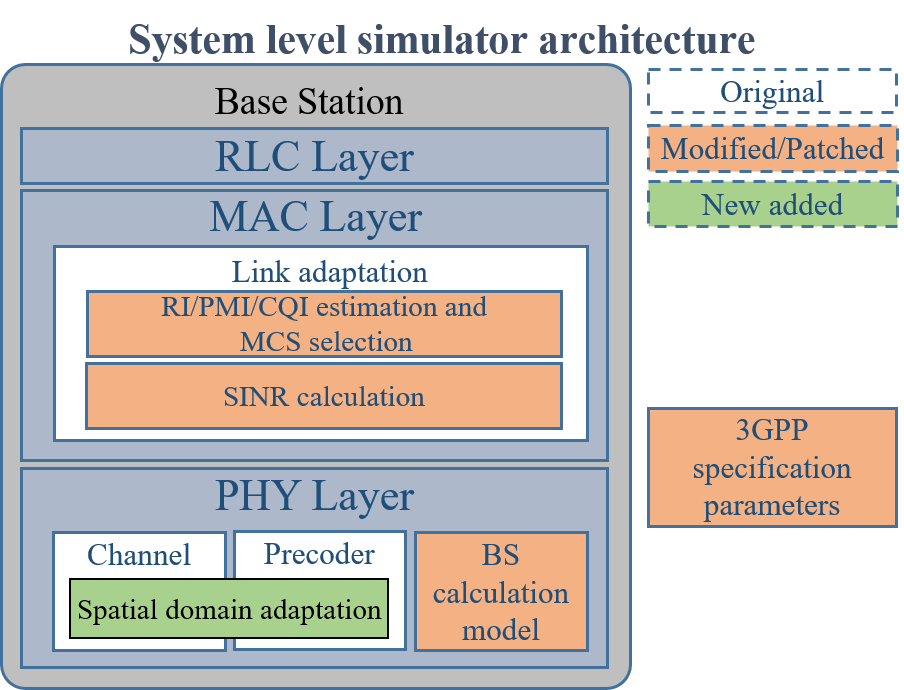
\includegraphics[width=0.85\textwidth]{figures/SLS_architecture.png}
    \caption{本研究擴充之 5G 系統級模擬器 (SLS) 核心架構圖}
    \label{fig:sls_arch}
\end{figure}

\subsubsection{網路拓撲與部署場景}
為建立具備高精確度、真實部署場景感與統計顯著性之實驗驗證平台，本研究採用符合 3GPP 國際標準規範之大規模系統級模擬（System-Level Simulation, SLS）環境進行效能評估。在網路拓撲規劃上，本研究部署一組由 7 個地理位置相鄰之基地台（gNodeB）所組成之細胞佈建，每個基地台包含 3 個獨立定向輻射扇區（Sectors），藉此共計建構 21 個服務細胞（Cells）以模擬真實多細胞環境。整體網路拓撲結構嚴格參考 3GPP TR 38.901 技術報告所建議之標準七細胞蜂巢式環狀部署架構（7-cell Ring Topology）\cite{3gpp_tr38901}，旨在透過多細胞重疊覆蓋之邊緣效應，有效考驗不同天線組態下之干擾抑制能力與空間複用效率。該基地台間之物理距離與地理佈局參數均依據標準規範進行嚴格建模，其具體佈局架構如圖 \ref{fig:network_layout} 所示。

\begin{figure}[htbp]
    \centering
    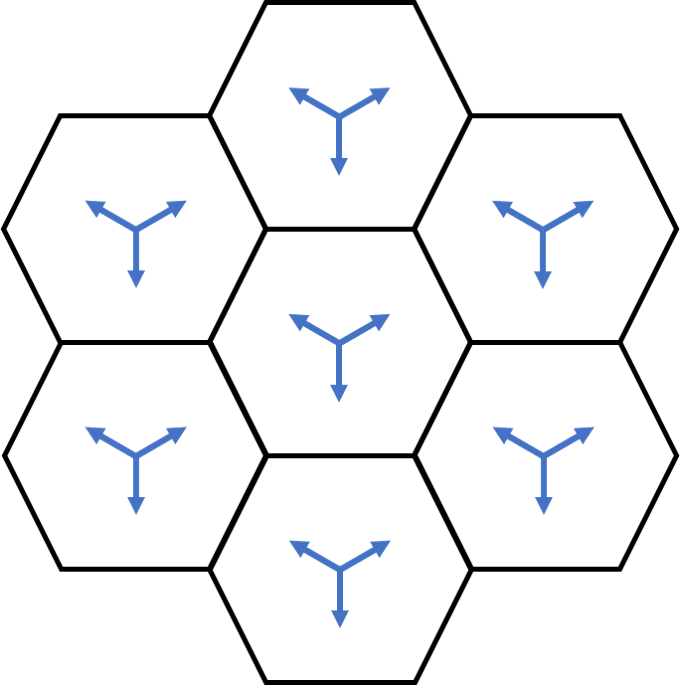
\includegraphics[width=0.7\textwidth]{figures/網路拓譜.png}
    \caption{7-cell Ring 蜂巢式網路佈局與模擬干擾場景拓撲示意圖}
    \label{fig:network_layout}
\end{figure}

此環狀拓撲之設計初衷與物理意義，在於模擬真實蜂巢式通訊網路中，細胞服務邊界極其複雜且高度動態的同頻相鄰細胞干擾環境（Inter-cell Interference）。特別是當基地台執行本研究所提之空間域適應（Spatial Domain Adaptation, SDA）策略，透過動態關閉實體層射頻鏈路（RF Chains）以進行基地台硬體能耗削減時，此拓撲結構能嚴謹且敏感地反映出服務細胞邊緣使用者（Cell-edge Users）在接收訊號品質 SINR（Signal-to-Interference-plus-Noise Ratio）受損下之服務品質（QoS）連鎖反應。

在使用者分佈與鏈路特性方面，本研究限定於下行鏈路（Downlink, DL）傳輸場景，並將 UE 設備於模擬區域內進行全域隨機分佈（Global Random Drop）。相較於於各細胞內強制固定使用者數量，此佈署模式更符合真實網路中用戶移動與分佈的隨機性，進而產生細胞間（Inter-cell）顯著的負載差異（Spatial Load Variation）。這種統計意義上的負載波動，對於驗證 SDA 機制在面對動態流量環境下之效能至關重要。同時，此佈署結合了符合 3GPP TR 38.901 規範之都會宏細胞（Urban Macro, UMa）真實通道模型 \cite{3gpp_tr38901}，模擬真實無線環境中之多徑衰落與干擾效應。透過此模擬框架，本研究旨在構建一個貼近實務佈署之測試平台，從而嚴謹地檢驗本研究所提之流量感知演算法在複雜網路場景下，如何兼顧節能增益與邊緣用戶服務品質之穩健性。

系統底層之硬體功耗係數對齊 3GPP TR 38.864 標準中所定義之 Category 1 Set 1 功耗模型基準 \cite{3gpp2023_tr38864}。在基地台天線架構方面，本研究採用基於 3GPP TS 38.802 標準之 64T64R Massive MIMO 陣列模型 \cite{3gpp_ts38802}，支援靈活之天線埠重組與空間域動態調適。基地台之下行最大傳輸功率設定為 49 dBm，載波頻率配置於 4.0 GHz，並採用 30 kHz 之子載波間隔（SCS）。在無線通道傳播模型上，本研究採用符合 3GPP TR 38.901 規範之都會宏細胞（Urban Macro, UMa）場景設定 \cite{3gpp_tr38901}。

流量模型採用 FTP Model 3，其讀取間隔為 500 ms，封包大小固定為 0.5 MB。在負載測試部分，設定低負載（$N_{UE/cell}=3$）與輕負載（$N_{UE/cell}=6$）兩種場景，UE 採用全域隨機分佈（Global Random Drop）以維持統計代表性。詳細之系統參數配置摘要如表 \ref{tab:sim_para} 所示：

\begin{table}[htbp]
\centering
\caption{Summary of System-Level Simulation Parameters}
\label{tab:sim_para}
\renewcommand{\arraystretch}{1.2}
\begin{tabular}{|l|l|}
\hline
\textbf{Parameter} & \textbf{Value / Assumption} \\ \hline
Network Topology & 7-cell Ring (21 cells total) \\ \hline
Carrier Frequency & 4.0 GHz \\ \hline
Max DL Tx Power & 49 dBm \\ \hline
Antenna Array Config. & 64T64R Massive MIMO \cite{3gpp_ts38802} \\ \hline
Subcarrier Spacing (SCS) & 30 kHz \\ \hline
Power Model & 3GPP TR 38.864 Cat 1 Set 1 \cite{3gpp2023_tr38864} \\ \hline
Channel Model & Urban Macro (UMa) \cite{3gpp_tr38901} \\ \hline
Traffic Model & FTP Model 3 (0.5 MB, 500 ms) \\ \hline
Load Conditions & Low ($N_{UE/cell}=3$) / Light ($N_{UE/cell}=6$) \\ \hline
\end{tabular}
\end{table}

\subsection{基地台功耗模型 (Base Station Power Consumption Model)}
本研究旨在透過空間域適應（Spatial Domain Adaptation, SDA）機制，在維持網路佇列穩定性之同時最小化基地台能耗。為了精確量化節能效益，本研究嚴格遵循 3GPP TR 38.864 技術報告 \cite{3gpp2023_tr38864} 所規範之 Category 1 Set 1 基準下行功耗模型（Active DL Power Consumption Model）。

依據標準規範，基地台在啟動下行傳輸狀態下之總輸入功耗 $P_{total}$ 由固定靜態功耗（Static Power）與動態功耗（Dynamic Power）線性組合而成：
\begin{equation}
P_{total} = P_{static} + P_{dynamic}
\end{equation}

為確保 SDA 機制在毫秒級時隙（TTI）內進行動態天線切換之即時轉換特性（Immediate transition），本研究將基礎靜態功耗 $P_{static}$ 設定為 TR 38.864 規範中之 Micro sleep 狀態基準值（即標準 Table 5.1-3 中之相對功率值 $P_3 = 55$），表示為：
\begin{equation}
P_{static} = P_{microsleep} = P_3
\end{equation}

動態功耗 $P_{dynamic}$ 則隨基地台之天線啟用規模與即時發射傳輸資源而變動。本研究採用縮放變數 $s_a, s_f, s_p$ 對其進行描述，其對齊 3GPP 標準之展開公式如下：
\begin{equation}
P_{dynamic} = s_a \cdot \left( P_{dyn, ante} + \frac{s_f \cdot s_p}{\eta(s_f, s_p)} \cdot P_{dyn, joint} \right)
\end{equation}

其中，公式內各縮放變數與效率函數之物理意義定義如下：
\begin{itemize}
    \item $s_a$：射頻鏈路啟動比例（Fraction of active TRxRUs）。此為本研究 SDA 機制之核心控制決策變數，代表實際啟用之 RF 鏈路數佔總天線埠數之比例。
    \item $s_f$：頻寬利用率比例（Occupied BW ratio），定義為實際佔用射頻頻寬與最大系統頻寬之比值。
    \item $s_p$：功率頻譜密度（PSD）調整係數，代表即時下行傳輸與基準配置間之 PSD 比例。
    \item $\eta(s_f, s_p)$：功率放大器（PA）之運作效率因子。依據標準規範，若系統採用雙值效率模型，當 $s_f \cdot s_p < 0.5$ 時，$\eta(s_f, s_p) = 0.76$；而在其餘高負載場景下則歸一化設定為 $\eta(s_f, s_p) = 1$。
\end{itemize}

動態功耗內部的兩大基準能耗分項 $P_{dyn, ante}$ 與 $P_{dyn, joint}$ 則由關鍵結構參數 $A$ 進行劃分，其計算方式定義如下：
\begin{align}
P_{dyn, ante} &= A \cdot (P_4 - P_{static}) \\
P_{dyn, joint} &= (1 - A) \cdot (P_4 - P_{static})
\end{align}

其中各項參數之基準數值與物理意義詳述如下：
\begin{itemize}
    \item \textbf{功耗分配權重 ($A$)}：依據 3GPP TR 38.864 基準配置，設定 $A = 0.4$。
    \item \textbf{天線依賴功耗分項 ($P_{dyn, ante}$)}：代表維持單一射頻鏈路與天線埠射頻元件基本工作狀態所需之基礎動態能耗。此部分能耗與實際發射功率無關，基於 $A=0.4$ 之設定，其佔據了動態基準差值的 40\%。
    \item \textbf{功率放大器相關能耗分項 ($P_{dyn, joint}$)}：在 3GPP 標準定義中，此分項表徵了與功率放大器（PA）直接相關之動態能耗。該項會隨著即時負載變數（頻寬利用率 $s_f$ 與發射功率密度 $s_p$）進行縮放，並受到 PA 運作效率因子 $\eta(s_f, s_p)$ 的動態調節。基於標準配置，其佔據了動態基準差值的 60\%（即 $1 - A = 0.6$）。
    \item \textbf{參考傳輸功耗 ($P_4$)}：為基地台全載發射下之下行參考功耗（Active DL），依照 Category 1 Set 1 標準設定其相對功率基準值 $P_4 = 280$。
\end{itemize}

為了確保模擬參數之產業公信力，本研究所採用之 3GPP TR 38.864 功耗狀態基準相對數值整理如表 \ref{tab:power_states} 所示：

\begin{table}[htbp]
\centering
\caption{Base Station Power States (TR 38.864 Category 1, Set 1)}
\label{tab:power_states}
\renewcommand{\arraystretch}{1.2}
\begin{tabular}{|l|c|}
\hline
\textbf{Power State} & \textbf{Relative Power ($P$)} \\ \hline
Micro sleep ($P_3 / P_{static}$) & 55 \\ \hline
Active UL ($P_5$) & 110 \\ \hline
Active DL ($P_4$) & 280 \\ \hline
\end{tabular}
\end{table}

基於上述之基地台功耗模型，為了客觀且量化地評估演算法之節能表現，本研究定義「節能率（Energy Saving Gain, ESG）」為核心效能評估指標。ESG 之計算方式為比較「未實施節能機制之基準狀態（Baseline）」與「實施 SDA 動態機制後」的長期平均功耗差異百分比，其數學定義如下：
\begin{equation}
\label{eq:esg}
ESG (\%) = \frac{\bar{P}_{total}^{baseline} - \bar{P}_{total}^{SDA}}{\bar{P}_{total}^{baseline}} \times 100\%
\end{equation}
其中，$\bar{P}_{total}^{baseline}$ 代表系統不啟用任何休眠或天線關閉機制（即始終維持 $s_a = 1$ 全天線開啟）下之時間平均總功耗；而 $\bar{P}_{total}^{SDA}$ 則為採用本研究所提之空間域適應機制後的平均總功耗。ESG 數值越高，代表演算法在維持網路運作之餘，成功削減的冗餘能耗越多。

透過上述對齊 3GPP 標準之數學建模與量化指標，基地台的即時動態功耗能精確與 SDA 決策變數 $s_a$ 產生連動。當SDA引擎在低負載場景下決定縮減天線組態（如 64T 降至 16T）時，$s_a$ 的比例調降將全面且成比例地削減公式中的天線基礎能耗與 PA 動態能耗。此一嚴謹的模型不僅符合業界規範，更為本論文後續建構 Lyapunov 漂移加懲罰（Drift-Plus-Penalty）最佳化問題中的能耗代價函數（Penalty Function）奠定嚴謹的理論基礎。
\subsection{通道狀態資訊與 Enhanced CSI 機制 (Channel State Information and Enhanced CSI Mechanism)}

在真實的 5G-Advanced 行動通訊系統中，細胞基地台係仰賴使用者設備（UE）定期回饋之通道狀態資訊（CSI）來執行鏈路適應（Link Adaptation）。然而，傳統的標準 CSI 回饋僅能反映基地台「當前運作天線維度」下的通道品質。

為了使本研究所提之決策引擎能在時隙（Slot）起始點，針對整個動作空間（16T、32T、64T）進行預期傳輸速率的提前估算，本研究於系統級模擬器（SLS）底層開發並實作了一套「增強型通道狀態資訊（Enhanced CSI）評估機制」。在通訊協定邏輯上，此機制之設計理念與 3GPP Release 18 網路節能（Network Energy Savings, NES）項目中探討之標準信令架構發展趨勢相呼應。

若依照傳統通道量測的方式要求 UE 回報多組天線組態之 CSI，傳統作法需由基地台發射多組實體導頻資源，這將造成嚴重的下行資源開銷（Overhead）。因此，依據 3GPP TS 38.214 \cite{3gpp_ts38214} 與 TS 38.331 \cite{3gpp_ts38331} 規範，本研究採用圖 \ref{fig:enhance_csi} 之架構：基地台僅發送單一全維度導頻訊號（Single CSI-RS），並透過配置 \textbf{CSI 報告子配置（CSI-ReportSubConfig）}，指示 UE 於本地端針對不同空間適應微調（Spatial Adaptation Pattern）進行平行之通道降維推估與回饋。

\begin{figure}[htbp]
    \centering
    
\includegraphics[width=0.6\textwidth]{figures/Enhance_CSI.png}
    \caption{多天線組態下之 CSI 測量機制 \cite{3gpp_ts38214}}
    \label{fig:enhance_csi}
\end{figure}

本研究所開發之 Enhanced CSI 模組，可視為此一前瞻標準機制在模擬環境下之合理簡化與等效建模。此設計在大幅節省導頻資源開銷的前提下，確保了決策引擎之輸入狀態具備高度的產業標準參考價值與工程可實現性。

\subsubsection{Enhanced CSI 觸發週期與時域限制}
本研究之系統級模擬（SLS）平台採用子載波間距（SCS）為 30 kHz 之配置（單時隙 $1 \text{ TTI} = 0.5 \text{ ms}$）。考量實體層運算開銷，系統並未在每個時隙盲目執行全動作空間之通道預估，而是將 Enhanced CSI 機制與標準系統之 CSI 回饋週期同步綁定，定義其量測觸發週期為 $T_{\text{CSI}} = 10 \text{ slots}$（即 5 ms）。

針對動態適應過程中「天線關閉時如何獲取通道資訊」的實務挑戰，本研究設計之 Enhanced CSI 係採用「週期性觸發」之運作機制。具體而言，當系統演進至 CSI 測量觸發點時，基地台會發送單一的全維度導頻訊號（Full-dimensional CSI-RS），此時系統內「所有活躍的使用者設備（UE）」皆會同步進行通道量測。

透過此週期性之全維度量測，UE 能夠於本地端「同時平行推估」多組候選天線配置（如 16T、32T、64T）下的通道狀態矩陣與預期頻譜效率。此機制不僅確保了決策引擎在每個週期皆能獲取所有天線配置的完整資訊，更在不額外增加導頻發射次數的前提下，達成了一次觸發、所有 UE 同時量測多組態的目標，完美解決了部分天線處於靜默狀態時無法獨立量測的技術瓶頸。

基於此時間限制，任何天線組態調適決策的觸發與生效，均嚴格受到 CSI 定期回饋時序的閉鎖約束。定義適應週期索引為 $k \in \mathbb{N}$，其基準決策錨點時隙為 $t_k = k \cdot T_{\text{CSI}}$。為了精確模擬真實基地台之控制流水線（Control Pipelining），本研究引入 CSI 量測偏移量 $T_{\text{CSI\_offset}}$ 與天線適應延遲 $T_{\text{SDA\_delay}}$，將 SDA 機制細分為以下三個階段：

\begin{figure}[htbp]
    \centering
    \includegraphics[width=0.95\textwidth]{figures/SDA_timeline.png}
    \caption{Enhanced CSI 量測點、SDA 決策點與切換生效延遲之時序關係圖}
    \label{fig:sda_timeline}
\end{figure}

\begin{enumerate}
    \item \textbf{Enhanced CSI 量測階段 ($uTTI = t_k - T_{\text{CSI\_offset}}$)}：
    當模擬時間演進至週期觸發點前夕（如圖 \ref{fig:sda_timeline} 範例中，決策錨點 $t_k = 10$ 對應之量測點為 $uTTI = 8$，$T_{\text{CSI\_offset}} = 2$ 個時隙），基地台於時隙起始處啟動通道探測程序。此階段針對所有活躍 UE 在各個候選天線組態下進行通道矩陣降維與頻譜效率預測，同時記錄此時隙之 MAC 層佇列積壓，確保決策引擎所需之輸入資訊具備跨層時序同步性。
    
    \item \textbf{SDA Decision 決策階段 ($uTTI = t_k$)}：
    基於前序時隙所收集之觀測數據，SDA 控制邏輯於決策錨點（$uTTI = 10$）進行運算，根據網路負載狀態與效能指標，執行天線組態之最佳化配置決策，並輸出該週期之目標天線組態指令 $a(k)$。此階段僅執行資源分配之求解，尚未觸發實體硬體之狀態切換。
    
    \item \textbf{硬體生效與組態更新 ($uTTI = t_k + T_{\text{SDA\_delay}}$)}：
    決策指令 $a(k)$ 產生後，系統進入歷時為 $T_{\text{SDA\_delay}}$ 的硬體切換空窗期（此範例中為 3 個時隙）。期間基地台維持舊有配置以確保傳輸穩定性。直至 $uTTI = 13$ 起始點，最新決策方正式灌入底層實體層，模擬器驅動通道矩陣執行降維屏蔽（Zero Masking），並同步更新功耗狀態模型，使得實體層正式運作之天線組態 $a_{\text{active}}(t)$ 更新為 $a(k)$。
\end{enumerate}

透過此一時域時序建模，基地台實際執行通道計算與功耗縮放時所採用之實體天線組態 $a_{\text{active}}(t)$ 滿足下式：
\begin{equation}
a_{\text{active}}(t) = a(k), \quad \forall t \in [k \cdot T_{\text{CSI}} + T_{\text{SDA\_delay}}, \, (k+1) \cdot T_{\text{CSI}} + T_{\text{SDA\_delay}} - 1]
\label{eq:sda_time_constraint}
\end{equation}

公式 (\ref{eq:sda_time_constraint}) 之核心用意在於將系統級模擬器底層之狀態暫存機制，轉化為控制理論中嚴謹的時域邊界限制式。起始點引入 $T_{\text{SDA\_delay}}$ 變數，精確建模了控制晶片發出決策後，射頻前端鏈路非即時切換（Non-instantaneous Transition）的硬體時滯特徵；結束點設定於下一適應週期生效點之前一刻（即減去單一時隙），其用意在於嚴格約束前後相鄰適應週期之邊界交接，消弭時間軸上的資訊冗餘與控制間隙，確保基地台實體狀態 $a_{\text{active}}(t)$ 在整體模擬時間軸上具備連續性與時域唯一性。

此一納入硬體時滯的非理想延遲系統建模，真實反映了動態天線調適在實務部署中所面臨之實體限制。這使得基地台無法在面對突發流量時「即時」改變天線能耗狀態，若控制演算法缺乏跨層的流量感知與預判能力，將在延遲空窗期內累積嚴重的佇列積壓，這也為本論文後續章節評估各種控制演算法在「網路節能」與「傳輸延遲」之間的權衡（Trade-off）績效，奠定了關鍵的時域評估基準。

最後，針對天線狀態頻繁切換所衍生的額外信令開銷（Signaling Overhead），實務上基地台可透過下行控制資訊（DCI）告知 UE 最新的天線與參考訊號配置。考量本研究之核心目標在於驗證 SDA 演算法之數學收斂性與跨層能效權衡，本論文目前暫將此一通訊配置機制視為理想假設，未將額外的信令開銷納入節能效果的折損計算中。

\subsubsection{空間域靜默之通道矩陣屏蔽建模 (Channel Matrix Masking)}

在實體層多天線通道建模中，定義單一使用者之全維度通道衰落矩陣為 $\boldsymbol{H}_{\text{full}} \in \mathbb{C}^{N_{Rx} \times N_{Tx, max}}$，其中 $N_{Tx, max} = 64$ 代表基準配置下之最大下行傳輸天線埠數，$N_{Rx}$ 為 UE 端之接收天線數。

依據 3GPP TR 38.864 標準所定義之空間域適應架構，本研究採用 \textbf{Type 1 (Subarray-1) 天線靜默機制}。選擇此機制主要基於以下三點實務與工程考量：首先，在目前學界與業界針對空間域適應（SDA）之研究中，Type 1 為最普遍採用之基準配置；其次，在通道狀態資訊（CSI）的量測開銷上，若採用其他天線縮減方式（如 Type 2），系統需為縮減後的天線陣列額外配置量測資源，而 Type 1 能夠直接將量測結果映射於同一個全維度矩陣中，大幅降低 CSI 的信令開銷；最後，考量到 3GPP TR 38.864 標準中 Set 1 所配置之 Non-codebook based 預編碼器（Precoder），採用 Type 1 以邏輯天線埠為單位直接關閉的作法，在現有運算與底層工程實作上較為直觀且具可行性。

如圖 \ref{fig:antenna_configs} 所示，當決策引擎欲評估較低維度之天線模式（由 64T 降階至 32T 或 16T）時，系統將以次陣列（Subarray）為單位，垂直關閉特定邏輯天線埠及其關聯之射頻鏈路（RF Chains）。


\begin{figure}[htbp]
    \centering
    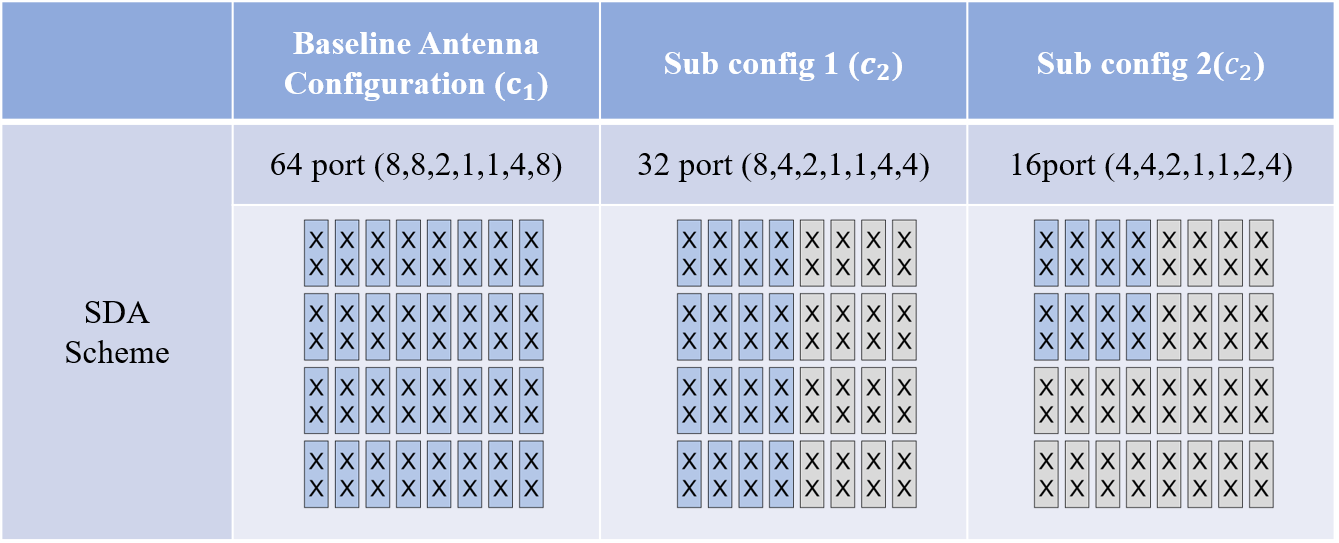
\includegraphics[width=0.7\textwidth]{figures/antenna_configs.png}
    \caption{空間域適應 (SDA) 候選天線組態與 Type 1 天線靜默機制之實體映射示意圖}
    \label{fig:antenna_configs}
\end{figure}

為維持系統維度之一致性與數學推導之嚴謹性，本研究並非直接刪減通道矩陣之行向量（Column Vectors），而是於系統級模擬（SLS）底層實作了等效之通道矩陣屏蔽技術（Zero Masking）。
\begin{figure}[htbp]
    \centering
    % width 已為您調整為 0.6\textwidth，若需再調整可直接修改數字
    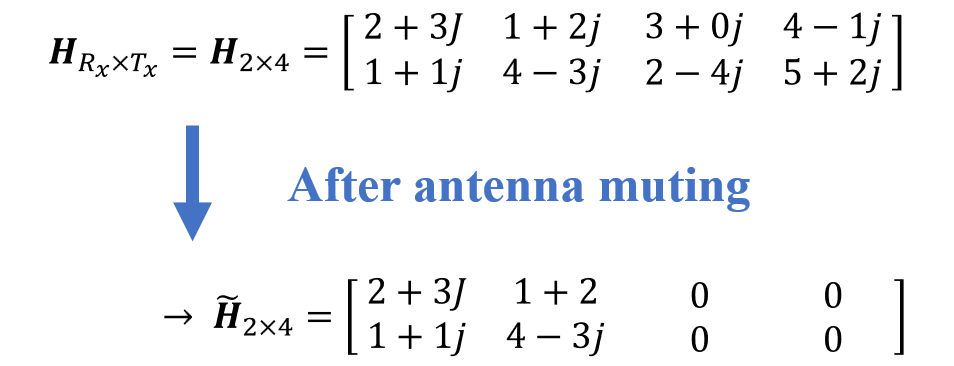
\includegraphics[width=0.6\textwidth]{figures/matrix_masking.png}
    \caption{基於 SDA 決策 $a(k)$ 之通道矩陣零屏蔽 (Zero Masking) 降維概念示意圖}
    \label{fig:matrix_masking}
\end{figure}

回到本研究之真實的系統維度，降維後之等效通道矩陣 $\tilde{\boldsymbol{H}}(a(k))$ 之數學表徵可定義為：
\begin{equation}
\tilde{\boldsymbol{H}}(a(k)) = \boldsymbol{H}_{\text{full}} \cdot \boldsymbol{M}_{a(k)}
\label{eq:matrix_masking}
\end{equation}

其中，$\boldsymbol{M}_{a(k)} \in \mathbb{R}^{N_{Tx, max} \times N_{Tx, max}}$ 為一全維度方陣，其對角線元素定義為 $\text{diag}(m_1, m_2, \dots, m_{64})$。遮罩係數 $m_i$ 的取值嚴格受控於當前之決策狀態：
\begin{equation}
m_i = 
\begin{cases} 
1, & \text{若第 } i \text{ 根天線埠在組態 } a(k) \text{ 下維持啟用} \\
0, & \text{若第 } i \text{ 根天線埠在組態 } a(k) \text{ 下被指定關閉}
\end{cases}
\end{equation}

公式 (\ref{eq:matrix_masking}) 之物理建模，精確且真實地反映了「Type 1 天線靜默（Antenna Muting）」之硬體關閉特徵。被屏蔽之天線單元不再發射任何導頻（Reference Signal, RS）與數據訊號能量，其對應之通道增益項在收端計算時完全歸零，從而動態改變了 UE 端所觀測到之幾何波束成型增益（Beamforming Gain）。透過此一嚴謹的矩陣屏蔽設計，模擬器得以在維持底層運算架構穩定的前提下，準確刻畫空間域適應（SDA）對於實體層通道傳輸品質之實質衝擊。

\subsubsection{通道品質映射與預期速率估測模型 (Channel Quality Mapping and Expected Rate Estimation Model)}
在獲得降維後之等效通道矩陣 $\tilde{\boldsymbol{H}}(a(k))$ 後，模擬器之實體層抽象化（Physical Layer Abstraction）模組將重新計算該 UE 於細胞內之有效訊號干擾雜訊比（Effective SINR），定義為 $\gamma(a(k))$。

為了將實體層之微觀通道指標，無縫轉化為媒體存取控制層（MAC）決策引擎所需之即時吞吐量參數，本研究採用符合 3GPP TS 38.214 規範 \cite{3gpp_ts38214} 之 5G-Advanced 256QAM 高階調變通道品質指標（Channel Quality Indicator, CQI）映射表進行頻譜效率轉換。

在 C++ 模擬器底層之實作中，本研究採用基於門檻值之離散查表邏輯（Threshold-based Discrete Mapping）。假設 3GPP CQI 映射表共包含 $N$ 個有效階層（Index $i \in \{1, 2, \dots, N\}$），每個階層對應一組解調所需之最低 SINR 門檻值 $\Gamma_i$ 與其可達成之頻譜效率 $E_i$（單位為 bits/symbol/Hz）。系統會藉由比對當前量測之 $\gamma(a(k))$，找出符合解調條件之最高 CQI 階層索引 $i^*$，其數學尋優條件可表示為：
\begin{equation}
i^* = \max \{ i \in \{1, 2, \dots, N\} \mid \gamma(a(k)) \geq \Gamma_i \}
\label{eq:cqi_index}
\end{equation}

選定最佳 CQI 階層後，其映射之頻譜效率函數 $f_{\text{map}}(\cdot)$ 即為該階層對應之固定效率：
\begin{equation}
f_{\text{map}}(\gamma(a(k))) = E_{i^*}
\label{eq:efficiency_mapping}
\end{equation}

最終，該 UE 在候選天線組態 $a(k)$ 下之預期下行傳輸速率 $R(a(k))$（單位為 bits/TTI）可估測為：
\begin{equation}
R(a(k)) = N_{\text{RE}} \cdot f_{\text{map}}(\gamma(a(k)))
\label{eq:expected_rate}
\end{equation}

式中，$N_{\text{RE}}$ 為系統配發予該 UE 之實體資源單元（Resource Elements）總數。透過此一嚴謹之 3GPP 查表映射機制，SDA 決策引擎得以準確預判「天線降維」對「實體層通道傳輸能力」的折損程度，並將此預期速率 $R(a(k))$ 作為後續李雅普諾夫最佳化演算法中，評估佇列積壓與延遲代價之核心輸入參數。



\subsection{李雅普諾夫最佳化理論基礎}
\label{sec:lyapunov_fundamentals}

在探討本研究之空間域適應（SDA）決策引擎前，本節將先介紹李雅普諾夫最佳化之一般性純數學理論框架 \cite{neely2010_stochastic}。在處理通訊網路之動態排程時，系統通常面臨資訊不對稱之困境：決策者無法預知未來封包到達之精確分佈，卻必須於當下做出保證系統長期穩定之決策。為在無未來資訊之前提下，解決「佇列穩定性」與「時間平均成本」間之多目標最佳化問題，本研究引入該理論作為底層演算法架構。

必須指出的是，儘管 3GPP TR 38.864 標準定義了天線域適應的實體架構與硬體切換機制，但並未明定基地台端應如何進行天線降維與復原的「決策解法」。在處理通訊網路之動態排程時，系統通常面臨資訊不對稱之困境：決策者無法預知未來突發封包到達之精確分佈，卻必須於當下做出保證系統長期穩定之決策。為填補此一標準上的技術空白，本研究引入李雅普諾夫最佳化理論作為底層演算法架構，其核心優勢在於能於「維持通訊品質（確保佇列收斂）的前提下最大化省電效益」，且具備無須預知未來流量即可進行線上即時決策之能力。

為在無未來資訊之前提下，解決「佇列穩定性」與「時間平均成本」間之多目標最佳化問題，本研究引入該理論作為底層演算法架構。

\subsubsection{系統擁塞度之量化：李雅普諾夫函數}
建立動態控制系統之首要任務，在於以數學模型量化系統當下之擁塞程度。考慮一離散時間之隨機佇列系統，令 $Q(t)$ 表示系統在時槽 $t$ 之佇列積壓長度。然而直接以 $Q(t)$ 作為指標並不足以反映系統瀕臨發散之急迫性。為此，李雅普諾夫理論定義一純量指標——李雅普諾夫函數 $L(t)$：
\begin{equation}
    L(t) \triangleq \frac{1}{2} Q(t)^2
    \label{eq:lyapunov_func_theory}
\end{equation}

於公式 (\ref{eq:lyapunov_func_theory}) 中引入平方項之核心目的，在於賦予控制系統「非線性懲罰」之數學特徵。在數學直覺上，可將李雅普諾夫函數 $L(t)$ 視為量化系統狀態偏離平衡點的二次方代價函數（Quadratic Cost Function）：當緩衝區中積壓之佇列長度 $Q(t)$ 處於低檔時，系統代價極小；然而當佇列長度成倍增加時，該代價將呈二次方級數（Quadratic Scale）急遽攀升。此一定義確保了當佇列積壓越嚴重時，最佳化控制引擎將產生越強大的排空驅動力（Draining Force），從而為維持網路強穩定性（Strong Stability）奠定嚴謹的數學基礎。
\subsubsection{多目標最佳化之權衡：漂移加懲罰框架}
為解決效能與成本間之絕對衝突，Neely 提出了漂移加懲罰（Drift-Plus-Penalty, DPP）框架。假設系統在時槽 $t$ 採取某一資源調配決策時，將產生對應之懲罰成本 $p(t)$（例如基地台之瞬時功耗）。該框架強制將 MAC 層的「運作成本懲罰」與「佇列穩定性」進行跨層級綁定，將控制目標轉化為在每個時槽瞬時最小化以下目標式：
\begin{equation}
    \text{Minimize: } \quad \Delta(t) + V \cdot \mathbb{E} [p(t) \mid Q(t)] 
    \label{eq:dpp_theory}
\end{equation}
公式 (\ref{eq:dpp_theory}) 中之 $V \ge 0$ 為一關鍵之控制權重參數（Control Parameter），其於理論框架中扮演調節樞紐之角色。根據李雅普諾夫最佳化定理，此一框架在數學上完美證明了系統之長期平均效能將嚴格遵循 $[ \mathcal{O}(1/V), \mathcal{O}(V) ]$ 的能效與延遲權衡邊界（Energy-Delay Trade-off Bounds）：

\begin{itemize}
    \item \textbf{能耗差距之收斂性 $\mathcal{O}(1/V)$：} 理論表明，系統實施演算法後之長期平均能耗成本，與全宇宙最省電之理論通用最佳解之間的差距，與控制參數 $V$ 成反比。當營運商將 $V$ 值微調得越大，此一差距便會以 $\mathcal{O}(1/V)$ 的邊際速率向零收斂，使演算法能極致發揮硬體以趨近省電天花板。
    \item \textbf{佇列延遲之理論上限 $\mathcal{O}(V)$：} 相對地，系統長期平均佇列長度（依據 Little's Law，其與排隊延遲呈線性正比）的最壞情況安全邊界，則與 $V$ 值成正比。這代表當系統為了追求極致節能而將 $V$ 值設定極大時，演算法將主動容忍網路封包延遲以 $\mathcal{O}(V)$ 的速率進行線性堆積。
\end{itemize}

此一定理為通訊系統注入了強大的閉環容錯機制。若控制參數 $V$ 趨近於零，決策引擎將無視功耗代價，全力壓制李雅普諾夫漂移 $\Delta(t)$，強迫硬體維持在高階天線組態以保障極致之低延遲；反之若 $V$ 設為高值，系統將對能耗懲罰項 $p(t)$ 高度敏感，進而理智地容忍佇列在安全容許區間內適度堆積，以換取深度的電力節省。最為關鍵的是，無論 $V$ 值如何變動，使用者的排隊延遲皆被強制鎖死在 $\mathcal{O}(V)$ 的線性邊界內，在數學層面徹底杜絕了佇列無限發散與網路癱瘓斷線之風險，為營運商在實施空間域適應（SDA）時提供了具備理論底氣的安全防護網。
\subsubsection{目標函數之上界推導與化簡}
雖然公式 (\ref{eq:dpp_theory}) 建立了多目標權衡機制，然而在真實隨機系統中，由於排程器無法預知未來的流量隨機波動，公式中的條件期望值在工程實務上無法直接求解。為了將此種高度依賴未來資訊之非因果難題轉化為可計算之數學模型，李雅普諾夫最佳化理論引入了「平方展開與求取上界」之數學技巧。

首先，根據控制系統對狀態變化趨勢之觀察需求，將公式 (\ref{eq:lyapunov_func_theory}) 之李雅普諾夫函數形式直接代入條件漂移項中，可將其明確展開為由當前與下一時槽佇列長度所構成之條件期望值形式：
\begin{equation}
    \Delta(t) = \mathbb{E}\left[ \frac{1}{2} Q(t+1)^2 - \frac{1}{2} Q(t)^2 \;\middle|\; Q(t) \right]
    \label{eq:drift_explicit}
\end{equation}

觀察公式 (\ref{eq:drift_explicit}) 可以發現，括號內部包含了未知的下一時槽佇列狀態 $Q(t+1)^2$。由於排程決策必須在當前時槽 $t$ 執行，此時未來的佇列積壓屬未知變數。為了將此一未來變數與基地台當前已知之佇列狀態 $Q(t)$ 建立物理規律上之數學關聯，本研究引入描述隨機佇列系統動態更新之特徵方程式：
\begin{equation}
    Q(t+1) = \max[Q(t) - \mu(t), 0] + \lambda(t)
    \label{eq:queue_general}
\end{equation}
其中，$\mu(t)$ 為系統在時槽 $t$ 決定之服務率，$\lambda(t)$ 為隨機封包到達率。公式 (\ref{eq:queue_general}) 中之 $\max$ 函數雖然確保了佇列長度不為負值之物理限制，然而在數學最佳化中卻引入了非線性且不可微之斷點特徵，導致公式無法直接進行解析與求期望值。

為突破此一數學瓶頸，本理論利用 $\left(\max[X, 0] + Y\right)^2 \le (X + Y)^2$ 之不等式特性，將公式 (\ref{eq:queue_general}) 兩邊進行平方展開。此操作之核心目的在於消除非線性算子，將原本難以求解之絕對等式放寬為具備高度代數運算性之數學上界：
\begin{equation}
    Q(t+1)^2 \le Q(t)^2 + \mu(t)^2 + \lambda(t)^2 - 2Q(t)\left(\mu(t) - \lambda(t)\right)
    \label{eq:queue_square}
\end{equation}

此一平方展開與求取上界技巧之關鍵效益，在於成功導出公式右側之交叉乘積項 $-2Q(t)\mu(t)$。該項在數學上直接將當前之系統擁塞壓力與演算法當下之控制決策建立直接之線性關聯，進而賦予演算法在佇列積壓時自動提升服務率之物理反饋自我調節機制。

隨後，將公式 (\ref{eq:queue_square}) 兩側同除以 $2$，並將當前狀態項 $\frac{1}{2}Q(t)^2$ 移項至不等式左側，即可精準顯現出與公式 (\ref{eq:drift_explicit}) 條件期望值內部核心結構完全對應之位能差值不等式：
\begin{equation}
    \frac{1}{2}Q(t+1)^2 - \frac{1}{2}Q(t)^2 \le \frac{1}{2}\left(\mu(t)^2 + \lambda(t)^2\right) - Q(t)\left(\mu(t) - \lambda(t)\right)
    \label{eq:drift_bound}
\end{equation}

對公式 (\ref{eq:drift_bound}) 兩側取給定當前狀態 $Q(t)$ 下之條件期望值，並代回公式 (\ref{eq:drift_explicit}) 中，即可得到李雅普諾夫漂移之初步條件上界。然而，由於其中的服務率 $\mu(t)$ 仍與當下的天線組態決策相關，無法直接視為常數。為了在數學最佳化過程中實現完全的決策解耦，本研究進一步引入系統的實體限制：由於基地台之封包到達率與硬體清空速率皆存在物理極限，令系統最大隨機到達率為 $\lambda_{max}$，最大硬體服務率為 $\mu_{max}$。因此，該時變平方項之預期值必受限於一絕對之硬體邊界，本研究將其定義為真正的常數上限 $B$：
\begin{equation}
    B \triangleq \frac{1}{2}(\mu_{max}^2 + \lambda_{max}^2)
    \label{eq:constant_B_def}
\end{equation}

利用此常數上限對時變平方項進行界定，並代回原始之漂移加懲罰目標函數公式 (\ref{eq:dpp_theory}) 中，即可導出綜合控制目標之理論上界界限：
\begin{equation}
    \Delta(t) + V \cdot \mathbb{E}[p(t) \mid Q(t)] \le B + V \cdot \mathbb{E}[p(t) \mid Q(t)] - Q(t) \cdot \mathbb{E}[\mu(t) - \lambda(t) \mid Q(t)]
    \label{eq:dpp_final_bound}
\end{equation}

經此轉換後，公式 (\ref{eq:dpp_final_bound}) 右側展現了即時最佳化求解之高度可行性。常數上限 $B$ 乃基於硬體規格所界定之固定實數，與演算法當下之天線組態決策完全無關；而未來之隨機封包到達率 $\lambda(t)$ 屬於外部網路行為之不可控外生變數，在數學最佳化過程中可與決策變數完全解耦。因此，為了最小化該理論上界，演算法無須任何未來預測資訊，僅需在每個獨立時槽中移除常數項與外生變數，針對當下可控之決策變數（成本 $p(t)$ 與服務率 $\mu(t)$）求解以下單步代數方程式：
\begin{equation}
    \text{Minimize: } \quad V \cdot p(t) - Q(t) \cdot \mu(t)
    \label{eq:lyapunov_magic}
\end{equation}
此一推導過程完美解釋了演算法如何將複雜的長期時變期望值問題，化簡為即時之線上最佳化運算，為後續空間域適應之應用建立了扎實之數學邏輯。

\subsection{基於李雅普諾夫之動態空間域適應決策模型}
\label{sec:lyapunov_sda_model}

在確立底層隨機最佳化之純數學通用框架後，本節將進一步探討如何將該抽象模型具體對應至 5G 基地台之空間域適應（SDA）節能場景中，以導出實作於媒體存取控制層排程器之線上決策方程式。

\subsubsection{系統變數對應與動作空間定義}
在 5G 動態多天線傳輸環境中，決策引擎必須在每個傳輸時間區間（TTI，即時槽 $t$）獨立為基地台決定最佳之天線開啟組態。本研究將通用最佳化變數，精確對應至實體層與協定層之隨機通訊參數：
\begin{itemize}
    \item \textbf{動作空間 $a(t)$}：代表基地台於時槽 $t$ 所採取之天線降維與靜默決策。其動作集合定義為離散之天線埠組態 $\mathcal{A} = \{16T, 32T, 64T\}$。
    \item \textbf{懲罰項 $p(t)$}：對應為基地台在採取動作 $a(t)$ 時，依據 3GPP 規範功耗模型所衍生之實體層總射頻與基頻運作能耗 $P_{total}(a(t))$。
    \item \textbf{服務率 $\mu(t)$}：對應為基地台在動作 $a(t)$ 與當下時變無線通道狀態下，系統排程器所能提供之各用戶實際資料傳輸速率 $R_n(a(t))$。
\end{itemize}

\subsubsection{SDA 線上最佳化方程式之建立}
透過上述變數對應，原本包含長期時變期望值之動態控制問題，得以被轉化為在每個獨立時槽中即時求解之單步代數最佳化問題。由於基地台此時唯一可控之核心變數為天線組態動作 $a(t)$，因此，本研究之 SDA 決策引擎簡化為在每個 TTI 線上尋求最佳天線決策動作 $a^*(t)$ 之問題：
\begin{equation}
    a^*(t) = \arg\min_{a(t) \in \mathcal{A}} \Big[ V \cdot P_{total}(a(t)) - \sum_{n \in \mathcal{N}} Q_n(t) \cdot R_n(a(t)) \Big]
    \label{eq:final_decision_sda}
\end{equation}
針對公式 (\ref{eq:final_decision_sda}) 中傳輸速率 $R_n(a(t))$ 與佇列長度 $Q_n(t)$ 相乘之減項，雖然在純數學推導上，其僅為李雅普諾夫漂移加懲罰框架化簡後（消去常數與外生變數）的代數結果，但其背後蘊含著極為關鍵的物理意義。此相乘項在控制系統中扮演了「佇列排空驅動力」的角色，用以平衡「傳輸效率（Data Rate）」與「佇列堆積（Queue Length）的延遲懲罰」。當特定用戶的佇列積壓越嚴重時，該乘積項的代數影響力隨之放大，迫使決策引擎優先選擇能提供高傳輸速率的天線組態（如 64T）以快速消化佇列；反之，若佇列長度極短，該乘積項的影響力大幅下降，引擎便會傾向最小化前端的功耗懲罰項 $V \cdot P_{total}(a(t))$，果斷切換至省電模式。

公式 (\ref{eq:final_decision_sda}) 完整展現了不依賴未來資訊之線上控制特徵。然而，傳統李雅普諾夫最佳化理論中將 $V$ 設為固定常數之假設，在面對 5G 具備高度隨機性與突發性之數據流量時，將遭遇工程部署上之理論瓶頸。若將固定常數 $V$ 設定過低，功耗懲罰項將失去制衡能力，導致輕載時喪失節能紅利；反之若設定過高，系統對功耗過度敏感，寧可容許佇列嚴重堆積亦不願擴展天線。此種剛性權重在流量劇烈轉渡時，極易引發決策遲滯與延遲發散，並在邊界負載下導致天線頻繁啟閉之乒乓效應。

\subsection{流量感知動態權重控制機制}
\label{sec:traffic_aware_v_control}

為克服固定權重引發之決策遲滯與切換乒乓效應，本研究提出一項核心創新機制：將傳統固定之控制參數 $V$ 改造為具備時間自我調適能力之流量感知動態權重控制函數 $V(t)$。其核心精神在於使基地台能夠根據當前網路之實際負載趨勢，動態改變演算法在節能提升與延遲防衛之間之代數渴望程度。

\subsubsection{流量感測指標與動態參數函數之建構}
為即時捕捉網路負載之時變特徵，本研究定義時槽 $t$ 之瞬時流量感測指標 $\rho(t)$。該指標透過排程器監測一個大小設定為 10 個 TTI 的滑動視窗（Sliding Window）內之平均封包到達率與系統最大服務容量之比值進行更新，數值範圍嚴格限制於閉區間 $[0, 1.0]$ 之間：

\begin{equation}
    \rho(t) = \min \left( \frac{A_{\text{avg}}(t)}{C_{\text{eff,max}}}, 1.0 \right)
    \label{eq:load_ratio}
\end{equation}

公式 (\ref{eq:load_ratio}) 中之各項組成變數與邊界算子之學術定義如下：
\begin{itemize}
    \item $\rho(t)$：代表無因次之系統即時有效負載率，用以表徵當前基地台無線資源被佔用與消耗的飽和程度。
    \item $A_{\text{avg}}(t)$：代表在特定歷史統計視窗內，基地台排程緩衝區所量測到之平均封包抵達速率，其計量單位為 bits/s。透過移動平均機制之平滑化運算，此參數能有效濾除短時間時槽內流量的隨機高頻漣波，提供穩定的負載基準。必須說明的是，此滑動視窗的大小設定會直接影響演算法對突發流量的敏感度（Sensitivity）：若視窗過大將導致決策反應遲緩，過小則易受雜訊干擾引發震盪。本研究在 MATLAB 邏輯沙盒階段曾對此參數進行多次評估與調校，目前的 10 個 TTI 設定為兼顧反應靈敏度與穩健性之最佳平衡值。
    \item $C_{\text{eff,max}}$：代表基地台在最大傳輸維度下，系統所能支援之理論最大有效服務容量限制，其物理單位為 bits/s。
    \item $\min(\cdot, 1.0)$：代表邊界飽和運算子，確保當網路面臨極端突發過載流量時，輸入決策系統之負載率能穩定收斂於臨界飽和邊界，防止後續權重計算數值發散。
\end{itemize}

為了使最大服務容量基準線 $C_{\text{eff,max}}$ 具備嚴謹的通訊實體層物理依據，本研究針對系統理論峰值頻譜效率上限值 $\eta_{\text{peak}}$ 進行標準對齊。參照 3GPP 實體層技術規範，最大理論峰值頻譜效率由下式進行嚴謹的純代數推導：
\begin{equation}
    \eta_{\text{peak}} = \nu_{\text{eff}} \cdot Q_m \cdot R \cdot (1 - \alpha_{\text{overhead}})
    \label{eq:peak_se_derive}
\end{equation}

公式 (\ref{eq:peak_se_derive}) 中之實體層核心通訊變數定義如下：
\begin{itemize}
    \item $\eta_{\text{peak}}$：代表系統之理論峰值頻譜效率上限，其計量單位為 bits/s/Hz。
    \item $\nu_{\text{eff}}$：代表多細胞部署環境下，受到同頻干擾與空間相關性等客觀實體鏈路瓶頸限制後，基地台排程資源塊上所能維持之有效統計峰值複用流數。此變數用以表徵多天線系統之實際空間域空間多工增益包絡線上限。
    \item $Q_m$：代表調變階數，用以表徵無線鏈路在極佳通道條件與高下行訊雜比下所能觸發之最高階調變模式，其計量單位為 bits/symbol。
    \item $R$：代表實體下行共享通道在最高排程 MCS 指標下之最大目標通道編碼率。
    \item $\alpha_{\text{overhead}}$：代表由下行實體控制通道、排程解調參考訊號及同步訊號區塊等實體層必要控制信令所佔用之資源開銷比例。
\end{itemize}

此理論峰值頻譜效率 $\eta_{\text{peak}}$ 建立了演算法資源調度之最高容量包絡線上限。藉由該實體層極限指標，結合基地台之最大可調配資源塊總數與排程有效折減係數，即可精確建構出符合真實通訊鏈路預算之最大有效傳輸容量 $C_{\text{eff,max}}$。關於上述各項實體層標準參數之具體模擬數值配置與校準結果，將統一彙整於第四章之模擬環境配置表中，此處專注於代數模型之建構。

在取得歸一化之即時網路負載狀態 $\rho(t)$ 後，演算法透過非線性調節函數對即時控制權重 $V(t)$ 進行動態自我修正，以實現控制目標的自適應切換：
\begin{equation}
    V(t) = V_{\text{min}} + (V_{\text{max}} - V_{\text{min}}) \cdot (1 - \rho(t)^{\gamma})
    \label{eq:dynamic_v}
\end{equation}

公式 (\ref{eq:dynamic_v}) 中之控制變數與自適應調控因子定義如下：
\begin{itemize}
    \item $V_{\text{max}}$：代表系統設定之節能優先權重閾值上限，用以在網路極度空閒時賦予能耗懲罰最高之加權，導引系統進入極致節能配置。
    \item $V_{\text{min}}$：代表系統設定之性能優先權重閾值下限，用以在網路資源飽和時將能耗懲罰弱化，確保佇列排空性能成為核心指標。
    \item $\gamma$：代表非線性調控因子，用以定義權重對於負載變化之響應靈敏度，其數值大小決定了權重衰減曲線之幾何曲率。本研究引入之非線性調控因子 $\gamma \ge 1$，能精準控制函數之敏感度響應曲線，避免負載微幅震盪時產生過度頻繁之反饋，自底層機制根除乒乓效應。
\end{itemize}


\subsubsection{動態權重控制之物理反饋解析}
將公式 (\ref{eq:dynamic_v}) 導出之動態參數 $V(t)$ 代回前述之固定權重核心決策方程式 (\ref{eq:final_decision_sda}) 中，最終之動態天線組態求解式轉換為：
\begin{equation}
    a^*(t) = \arg\min_{a(t) \in \mathcal{A}} \Big[ V(t) \cdot P_{total}(a(t)) - \sum_{n \in \mathcal{N}} Q_n(t) \cdot R_n(a(t)) \Big]
    \label{eq:final_decision_dynamic_v}
\end{equation}

公式 (\ref{eq:final_decision_dynamic_v}) 之動態最佳化反饋迴圈，其精妙之物理控制邏輯可依系統負載狀態客觀剖析如下：
\begin{itemize}
    \item \textbf{極低負載區間}：當網路處於極輕載狀態時，平均封包抵達速率遠小於最大承載容量，$\rho(t) \to 0$。非線性調節項趨近於 1，權重 $V(t)$ 被推升至上限值 $V_{\text{max}}$。此時公式 (\ref{eq:final_decision_dynamic_v}) 中之功耗懲罰項之代數權重放大至極致，引導決策引擎優先選擇低功耗天線組態（如 16T），最大化系統能源效率。
    \item \textbf{非線性過渡區間}：當網路流量增長時，調控因子 $\gamma$ 發揮緩衝效果。在流量增加初期，$V(t)$ 維持在相對高檔，延長低傳輸維度運作時間。一旦負載突破臨界門檻，權重 $V(t)$ 進入陡峭衰減軌跡。此預警機制使系統在佇列嚴重壅塞前平滑調降能耗權重，完全消弭固定閾值切換之乒乓效應。
    \item \textbf{重負載與飽和區間}：當突發流量爆發，網路負載率逼近飽和（$\rho(t) \to 1.0$）。非線性映射項歸零，權重降至下限 $V_{\text{min}}$。佇列權重服務增益項轉為決策核心，演算法主動放寬能耗限制，果斷切換至最大組態（如 64T）。藉由大規模多天線之多工增益，以最大速率排空佇列積壓，捍衛終端用戶之服務品質（QoS）。
\end{itemize}

進一步探討本研究所提之動態權重機制，其另一項關鍵優勢在於能有效避免傳統方案中常見的「佇列延遲發散（Queue Delay Divergence）」現象。在傳統基於負載的啟發式演算法（Load-based Heuristics）中，決策引擎過度依賴「過去一段時間內的平均負載」作為判斷基準。當真實網路中遭遇極端的突發流量（Burst Traffic）且該波流量瞬間結束時，系統會因歷史觀測視窗的滯後性（Time Lag）而無法及時反應，進而產生盲目且頻繁的天線開關切換，即所謂的「乒乓效應（Ping-pong Effect）」。

這種盲目的狀態切換會導致嚴重的資源錯位：在真正需要高傳輸速率來排空積壓封包的瞬間，系統可能因平均負載指標下降而提早切換回省電模式（如 16T）；而在佇列已清空、無數據可傳時，卻又因先前的負載記憶而維持在高耗能組態（如 64T）。這種傳輸資源與實際需求的嚴重錯位，使得瞬間爆增的佇列無法被有效且連續地消化，最終引發佇列延遲的嚴重發散。相反地，本研究之公式 (\ref{eq:final_decision_dynamic_v}) 直接將「瞬時佇列長度 $Q_n(t)$」作為驅動決策的核心乘積項，實現了零滯後的即時反饋，從物理機制上徹底斬斷了乒乓效應與延遲發散的因果鏈。
\subsubsection{演算法實作流程與時序對齊}
本研究提出之決策演算法運作於基地台媒體存取控制（MAC）層，依據通道狀態資訊（CSI）更新週期執行閉迴路控制。整體架構由流量感知、最佳化決策與延遲緩衝執行三個模組組成，詳細步驟如演算法 \ref{alg:sda} 所示：

\begin{algorithm}[htbp]
\caption{Traffic-Aware Lyapunov-based SDA Algorithm}
\label{alg:sda} 
\centering

\includegraphics[width=1\linewidth]{SLS_algorithm.png}
\end{algorithm}

\paragraph{一、 演算法步驟執行流程}
演算法之具體運作邏輯可詳細拆解為以下三個實作階段：
\begin{itemize}
    \item \textbf{系統狀態估測（步驟一）}：當系統時脈滿足 CSI 更新週期條件時，流量感知模組會讀取特定統計滑動視窗內之平均封包抵達速率 $A_{\text{avg}}(t)$，並與基地台之最大有效傳輸容量 $C_{\text{eff,max}}$ 相除以求得歸一化負載率 $\rho(t)$。隨後，將此負載率代入非線性調節函數中，計算並更新當前決策點之即時能耗控制權重 $V(t)$。
    \item \textbf{漂移加懲罰最小化（步驟二）}：決策引擎擷取當前所有活躍行動用戶積壓之佇列長度 $\{Q_n(t)\}$。針對合法動作空間內之離散天線組態動作 $a \in \{16T, 32T, 64T\}$，決策引擎聯立評估該動作下之基地台功耗 $P(a)$ 與各用戶之預估可達速率 $R_n(a)$。透過將佇列長度作為速率之加權乘積，求得漂移加懲罰目標函數值 $Obj(a)$，最終藉由 $\arg\min$ 算子選出使該目標函數值最小之天線配置動作 $a^*(t)$。
    \item \textbf{時序延遲緩衝執行（步驟三）}：考量基地台射頻鏈路與信令重組之物理切換時延，演算法將所求得之最優天線組態 $a^*(t)$ 存入延遲緩衝排程器中，並排程至未來時隙 $t + T_{\text{SDA\_delay}}$ 生效。當模擬時脈演進至該指定時隙時，基地台即透過天線遮罩機制執行相對應之硬體埠配置。
\end{itemize}

\paragraph{二、 系統級模擬器實作時序對齊說明}
在系統級模擬器（SLS）之 C++ 程式碼實作層面，函數的底層執行順序與上述由演算法 \ref{alg:sda} 所建立的純數學理論邏輯流存在結構性的微調。圖 \ref{fig:sls_workflow} 完整展示了 SLS 模擬器在單一 TTI 時脈演進下的實際程式呼叫流程與 SDA 控制模組的無縫嵌合關係。

\begin{figure}[htbp]
\centering
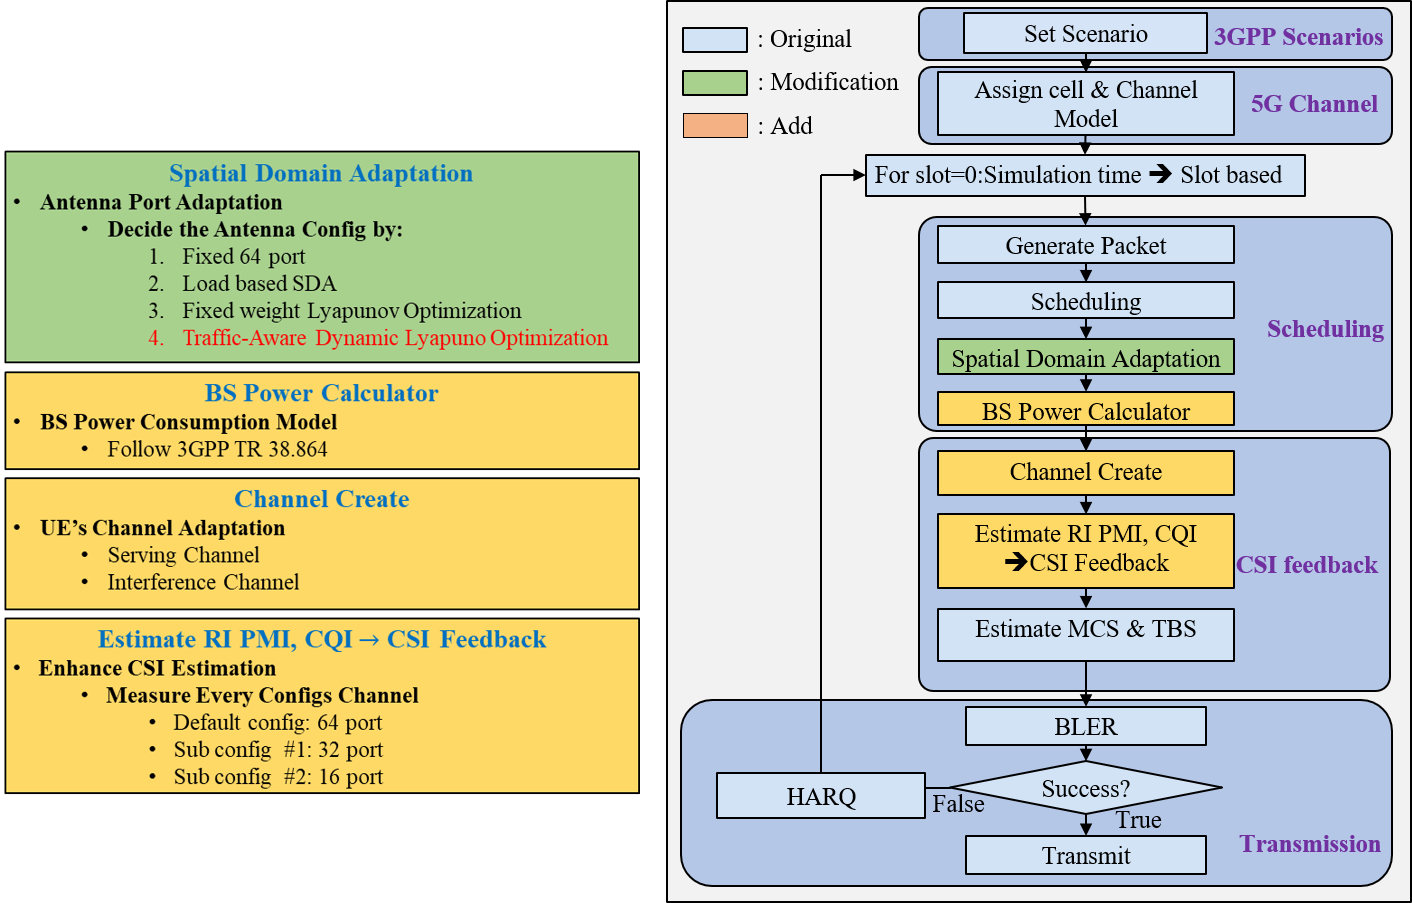
\includegraphics[width=1\textwidth]{figures/SLS_workflow.png}
\caption{5G SLS 模擬器底層主迴圈與動態天線調適模組實作執行時序圖}
\label{fig:sls_workflow}
\end{figure}

值得注意的是，此一流程時序圖不僅用以表徵純理論演算與實務模擬之間的時序交疊差異，更具體呈現了本研究為了將 SDA 決策引擎引入既有平台，於 PHY 層與 MAC 層交界處所全新開發之獨立控制模組，以及針對底層天線埠映射與通道衰落矩陣執行零屏蔽降維所進行之軟體架構改動。此一圖示直觀地勾勒出新開發模組與既有標準模擬環境之間的資訊介接通路。

理論偽代碼所呈現的順序，是基於控制理論的因果決策鏈，意即系統必須先觀測宏觀負載、更新最佳化權重，再計算目標函數並下達配置決策。然而，在時脈驅動的真實 SLS 模擬器中，程式的執行順序必須遵循資料邏輯上的先後相依關係。

由於本研究啟用了全動態傳輸層數（Rank）自適應機制，在動態 Rank 模式下，每個天線動作 $a$ 所對應之預估可達傳輸速率 $R_n(a)$ 並非固定的常數因子，而是高度相依於當前多細胞干擾、空間幾何通道實現以及鏈路層抽象化映射後所得到的即時訊號雜訊比。從行動通訊的實體鏈路限制來看，通道狀態資訊（CSI）的下行導頻量測、用戶終端之通道估測運算、上行鏈路控制通道回傳，乃至於基地台端的解調讀取，本質上屬於一跨越複數時槽的跨層閉迴路時延程序，絕無可能在單一時槽之內瞬間完成整體控制流程。

因此，模擬器的軟體架構必須採取底層資訊優先蒐集之因果相依邏輯：若實體層未先執行通道建模與訊雜比估算，MAC 層的決策引擎便無法獲得有效的速率估測矩陣 $\{R_n(a)\}$ 作為輸入引數，這將導致步驟二的李雅普諾夫目標函數 $Obj(a)$ 缺乏數據基礎而無法求值。基於此一通訊實體時滯與資料依賴性限制，SLS 原始碼的函數執行序列調整為：先更新實體層通道狀態資訊、蒐集 MAC 層佇列積壓，隨後在滿足控制週期時觸發 SDA 決策核心以求解最小化問題，並將決策寫入延遲緩衝排程器。此一基於實體物理限制與數據依賴性所進行的時序重組，在數學優化邊界上與理論完全等價，並確保了演算法在時脈模擬器中的精確收斂。

\paragraph{三、 演算法計算複雜度分析}
本演算法將複雜的長期時間平均最佳化目標，成功解耦為每個決策週期內之瞬時最小化求解問題。在計算開銷方面，由於動作空間 $\mathcal{A}$ 僅包含三種離散天線維度組態，決策引擎在每個更新週期內僅需執行三次目標函數之代數評估與比較。因此，該演算法之運算複雜度嚴格收斂於常數階 $\mathcal{O}(|\mathcal{A}|)$。此開銷與系統內部之行動用戶總數完全解耦，具備極低之運算與記憶體開銷，適宜嵌入現有基地台之排程晶片中即時執行。


